
\label{sec:sl}

{\it Phil Marshall, Tommaso Treu, Curtis McCully and Eric Linder}

Our ability to do cosmography with either time delay lenses or multiple
source plane ``compound'' lenses is dependent on follow-up observations
to constrain the mass models: without these data, strong lenses will not
be able to be used for precision cosmology. In this section we outline what will be
required in order for us to be able to exploit the LSST strong lens sample.


% ----------------------------------------------------------------------

\subsection{Science Goals}

% {\it Describe your science goals here, as in the scientific justification of an NOAO proposal. If you have multiple science goals, you can either describe them all here, or replicate the science, technical, and capabilities sections for each goal. Just create one summary table for the entire program.}

%NOAO guidelines:
%
%The scientific justification should explain the overall goals of
%your program in the context of your field, as well as the importance
%of your program to astronomy.
%Writing a good scientific justification is an art.  It takes
%skill and practice.  And it requires a good scientific idea.
%This last you must supply but a few general guidelines
%about proposal writing might still be helpful...
%
%\begin{itemize}
%\item
%State succinctly and clearly the problem you are trying to solve
%and the progress that will be made toward doing so if the proposed
%observations are successful.  If the review panel members have to work hard
%even to understand what you want to do, they are unlikely to be
%sympathetic to your proposal.
%
%\item
%Explain clearly why the project is important and how it
%relates to the broad context and important issues in your field.
%Many proposals focus too tightly on a specific observational
%goal (e.g. ``measure the velocity dispersion of this cluster of galaxies'')
%without explaining why it is important or how it relates to a
%significant question about the Universe.
%
%\item
%Be specific.  If your observations will ``constrain theoretical
%models,'' then discuss what will be constrained and why those
%constraints matter.  Make sure the review panel understands exactly why
%the observations you propose will make a difference in your field,
%and exactly how the observations will refine or
%require changes in the theory.
%
%\item
%Keep it simple.  Try to focus on the central idea of your proposal.
%Complex arguments are hard to explain and hard for the panel members to follow.
%Distracting tangential arguments obscure the theme of your proposal.
%
%\item
%Include a figure to help explain what you want to do.  Sample
%data or model predictions shown in a figure often help clarify
%complex arguments for the panel members.
%
%\item
%Keep it short.  Never exceed a page for the text of the scientific
%justification, and never reduce the font size.  It may even help to
%be a little under a page, and increase the font size a little!
%Organize your presentation with paragraphs, headings, and bullets
%so it is easy to read.

\label{sec:sl_just}

The primary route to cosmology from strong lensing is time delays in
galaxy-scale lensed quasars and supernovae. Galaxy scale compound lenses
(i.e. systems with two sources at different redshifts) have also been
suggested. We expect to be able to compile samples of several hundred lensed AGN
and lensed SN systems with accurately measured LSST time delays \citep{LiaoEtal2015},
and dozens of compound lens systems \citep{Collett2015}.\footnote{The
LSST strong lens sample will be compiled semi-automatically, using algorithms developed and implemented by the LSST DESC that are
run on the DM Level 1 and 2 data products, and whose products are then assessed -- including visually -- by the DESC analysis team. Some of the technology involved in this process could be developed and operated in collaboration with the Galaxies and Strong Lenses collaborations.}

Figure~\ref{fig:sl_forecast}, reproduced from \citet{Coe+Moustakas2009}
shows approximate forecast cosmological  parameter constraints from a
sample of 100 lenses, where each provides a  time delay distance
accurate to 5\%. Two lenses to date have been  shown to provide 6\%
distance precision \citep{SuyuEtal2014}: this was only  achievable with a
combination of deep, high resolution imaging from HST (to enable the
Einstein rings to be modeled), and high fidelity spectra from 10-m class
telescopes yielding lens velocity dispersions that anchor the mass
model. Without these follow-up data, the mass models can only be
constrained to 20--30\% accuracy: {\it for this cosmological probe, the
optical and infrared follow-up observations are essential.} LSST will
simply provide the opportunity, via a large sample of accurately
measured time delays.

\begin{figure*}[!t]
    \centering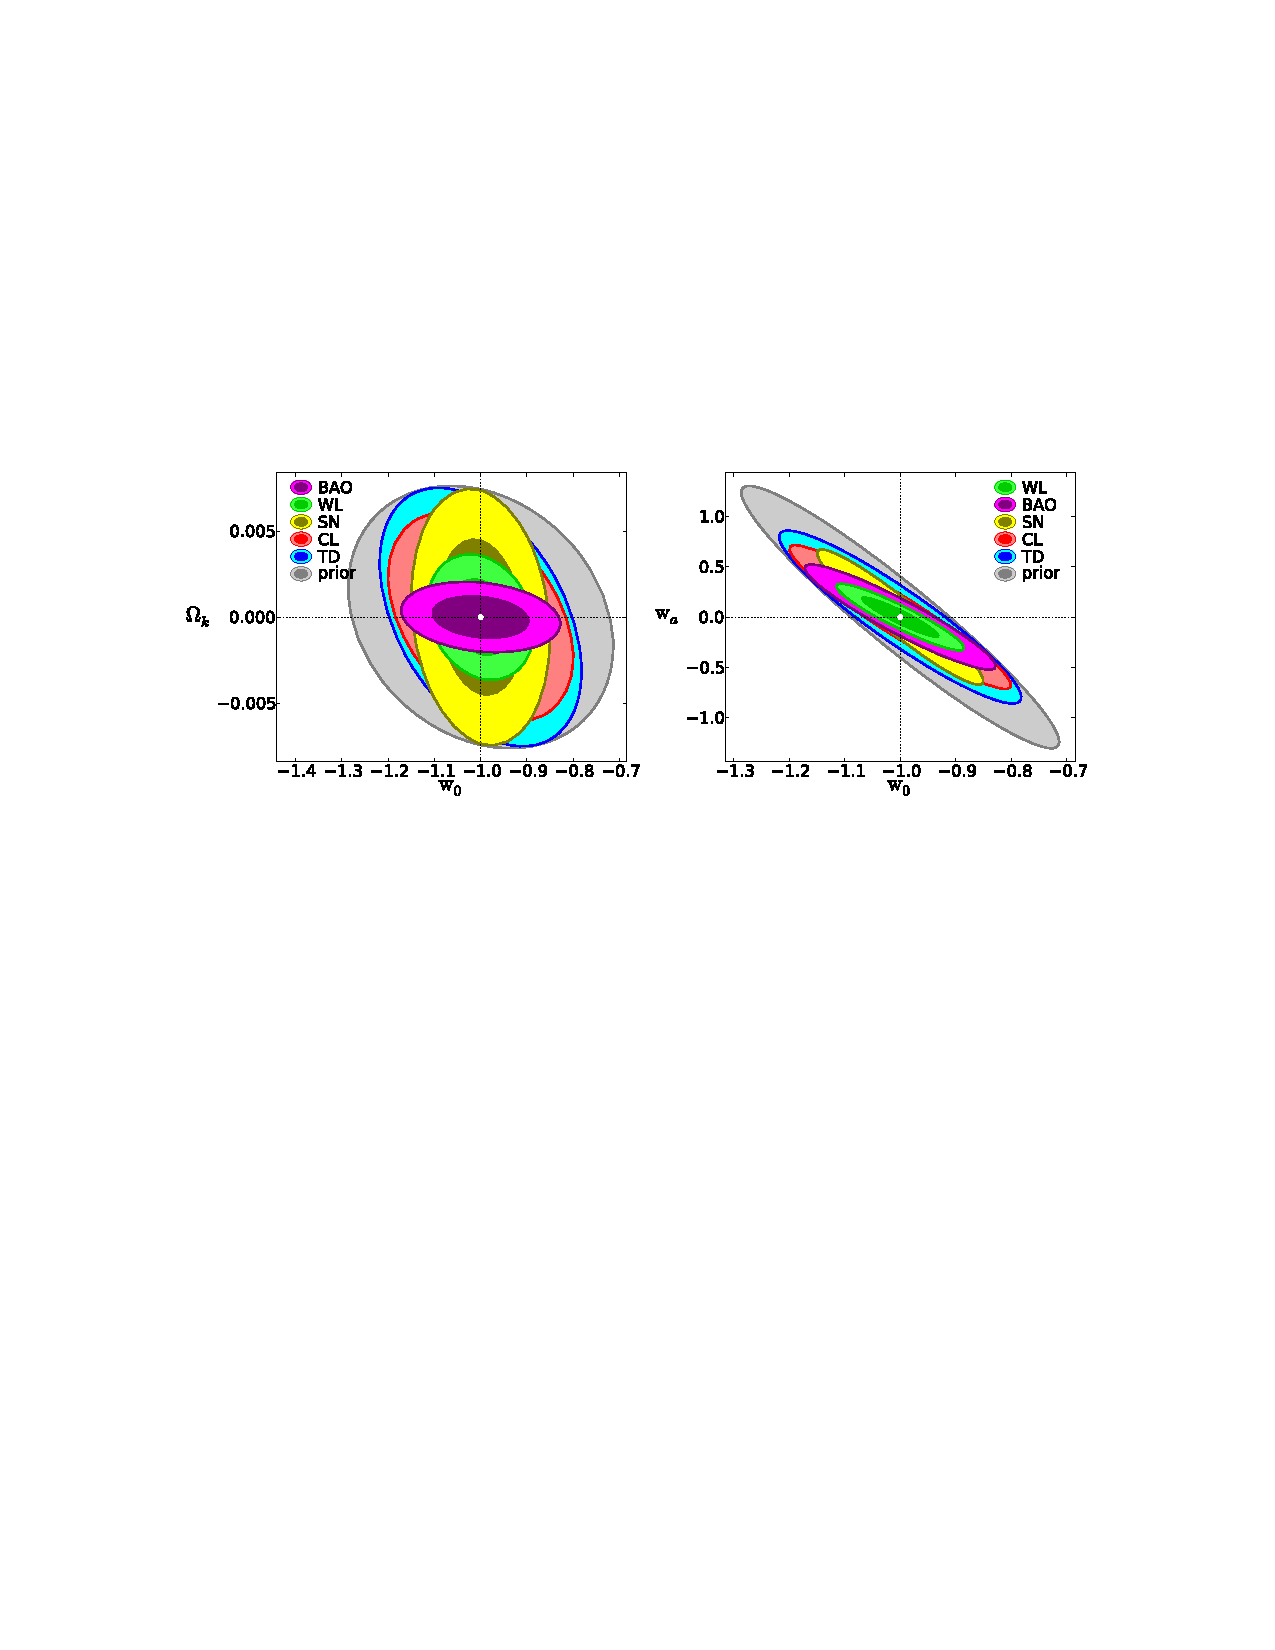
\includegraphics[width=0.9\linewidth]{figs/Coe+Moustakas2009_Figure14.pdf}
    \caption{LSST time delay lens cosmological parameter forecasts (`TD', blue ellipses)
    compared to forecasts from the Dark
    Energy Task Force \citep{DETF} for four other Stage IV probes of cosmology: Baryon Acoustic Oscillations (`BAO'); Weak Lensing (`WL'); Type Ia Supernovae (`SN'); and Cluster counts (`CL').  The parameters considered are the Dark Energy equation of state parameter $w=P/\rho$ evaluated today ($w_0$); its evolution with the scale factor of the Universe in a linear model, i.e. the parameter $w_a$ for the model $w(a) = w_0 + w_a\times(1-a)$; and the curvature of the Universe expressed as a fraction of its critical density, $\Omega_k$.   The prior probability distribution assumed for cosmological parameters is shown in grey.
    A sample of 100 lenses is assumed, each one
    providing a 5\% accurate time delay distance. Figure reproduced from
    \citet{Coe+Moustakas2009}.}
    \label{fig:sl_forecast}
\end{figure*}

% ----------------------------------------------------------------------

\subsection{Technical Description }

% {\it Give a technical description of your program, describing e.g., sample size and properties, justification of spectral or spatial resolution, wavelength, target density, etc.}


%NOAO guidelines:
%The review panel looks to this section to find out about the overall
%strategy of your observational program.  Why do you need the telescopes
%and instruments you request? How are your targets selected?
%Why do you need spectroscopy or imaging, and what measurements will
%you make from the data?  Why is your approach to be preferred over
%some other approach, what must the minimum sample size be to achieve
%your scientific goals (and why), and why are your
%observations likely to be better than previous work in the field?

To be useful as probes of cosmological distances, galaxy scale lenses
need very well constrained mass models. These constraints will come from
two types of targeted follow-up observations:\footnote{
We note that these observations would be taken after targeted optical
spectroscopy to get the redshifts of the deflector and source galaxies.
This can be done at relatively low resolution, but the wider the
wavelength range the better: we will need 3500--10000 Angstroms in the
optical, and maybe a triplespec-like instrument covering the JHK bands
in the IR. Some redshifts may come from overlapping spectroscopic survey
observations, with the systems appearing as composite absorption and
emission line galaxy spectral components. Some of the targeted
spectroscopy could be done at 10-m class facilities.}
\begin{enumerate}
    \item {\bf High Resolution Einstein Rings Imaging} due to the
    source AGN or SN host galaxy. Image quality of $\sim0.1$" or better
    provides the Einstein ring constraints on the lens mass model
    density profile slope (via the arc thickness) that are
    needed to turn each of these systems into a  5\% precision distance
    \citep{MengEtal2015}.
    \item {\bf Spatially-Resolved Spectroscopy of the Lens Galaxy,} enabling
    measurement of the stellar velocity dispersion field to break the
    degeneracy between the predicted time delays and the lens mass
    density profile, calibrating each system to enable it to provide a
    4\% accurate distance.
\end{enumerate}

We now assess the technical  requirements of each of these observations.

{\bf 1. High Resolution Einstein Ring Imaging}:

$\bullet$ Spectral coverage and resolution: imaging in two or three
bands is recommended, to enable clean lens galaxy subtraction.

$\bullet$ Angular resolution: the higher the resolution the better, but
at least $0.1$~arcsec FWMH.

$\bullet$ Depth: the host galaxies of the lensed sources are faint (mag
23--25). Brighter sources will be prioritized when compiling the
follow-up sample, based on analysis of the survey images, and exposure
times of up to 1 hour would be considered, with fainter systems being
discarded \citep{MengEtal2015}.

$\bullet$ Field of view: at least 4~arcsec, to capture the Einstein
ring without dithering.


{\bf 2. Spatially-resolved Spectroscopy of the Lens Galaxy}:

$\bullet$ Spectral coverage and resolution: $R\approx4000-5000$  over a
wavelength range of 1.0--2.2 microns (to cover the Calcium triplet at rest frame
$\sim8500-8700\AA$, or CO at $1.5-1.6\mu$m).

$\bullet$ Angular resolution: 0.1--0.2~arcsec, to resolve the lens galaxy well.

$\bullet$ Depth: the lens galaxies will have brightness in the range
19--22 magnitudes. Again, exposure times of an hour or less will be
considered, with fainter systems being discarded.

$\bullet$ Field of view: at least 4~arcsec, to capture the lens galaxy
within the Einstein ring without dithering.

The above requirements are derived from end-to-end simulations of the
kind carried out by \citet{MengEtal2015}, which will be refined before
proposals to next generation facilities are submitted.

% ----------------------------------------------------------------------

\subsection{Needed Capabilities and Estimate of Demand}

% {\it Describe the needed capabilities and demand (e.g., estimate of observing time) that flow down from the science and technical considerations. If applicable, describe the time critical nature of the required capabilities (do you need to have the capabilities while LSST is carrying out the survey or can you do the follow up later?)}

AO-assisted imaging and integral field spectroscopy on GSMTs would be
best for providing the lens mass model constraints detailed in the
previous section.  We will need capabilities such as those currently
available on Keck, and that will be available on all three of GMT, TMT
and E-ELT (albeit with somewhat different technical specifications).
OSIRIS on Keck is the current best option, even though the field of view
is a bit too small and the current AO system at Keck has relatively low
strehl at 1$\mu$m. The Keck system will be upgraded, but TMT should be
much better: IRIS on TMT would provide the capability we need. Similar
data would be needed for the compound lenses.

The light curves will be accumulated by LSST over the lifetime of the
survey, but we expect accurate cosmography to be possible after the
first 5 years.  Prior to this, the same facilities could be used to good
effect improving the models of lenses found in shallower precursor
surveys such as DES, KIDS and HSC. We expect to have good time delays
for about 30-40 systems before the LSST survey begins: these would be
the targets for high resolution follow-up before 2024, with an
additional 60-70 targets coming from the LSST survey being pursued
between 2024 and 2028 and beyond. The demand is therefore likely to be
around 10-20 systems per year; we assume the higher value below, to help
with planning.

While the targeted observations outlined below would be narrow field,
they would enable a considerable amount of ancillary science, notably in
the areas of dark matter substructure (from perturbations to the imaged
rings) and AGN host galaxy structure.  To summarize, the needs for LSST strong lensing studies are:

{\bf 1. High Resolution Einstein Ring Imaging}:

$\bullet$ Proposed facilities: GSMTs, JWST. 10m-class telescopes for
brighter rings.

$\bullet$ Observations needed: Targeted snapshot (e.g.\ 200--2000
second exposure time with TMT) imaging in the optical and near infra-red.

$\bullet$ Total time required: $\sim30$~hours, depending
on balance between facilities (assuming 20~mins per system, on average),
or $\sim 6$ hours per year.

{\bf 2. Spatially-resolved Spectroscopy of the Lens Galaxy}:

$\bullet$ Proposed facilities: GSMTs, JWST.

$\bullet$ Observations needed: IFU spectra in the near infra-red.

$\bullet$ Total time required: $\sim100$~hours, depending
on balance between facilities (assuming 60~mins per system, on average),
or $\sim 20$ hours per year.

Both the imaging and spectroscopy will be critical for LSST strong lensing cosmology, and hence very important for LSST cosmology considered as a whole.
